
\usetikzlibrary{shapes.geometric}
\usetikzlibrary{calc}
\definecolor{darkBlue}{RGB}{40,55,155}

\resizebox{0.4\textwidth}{!}{
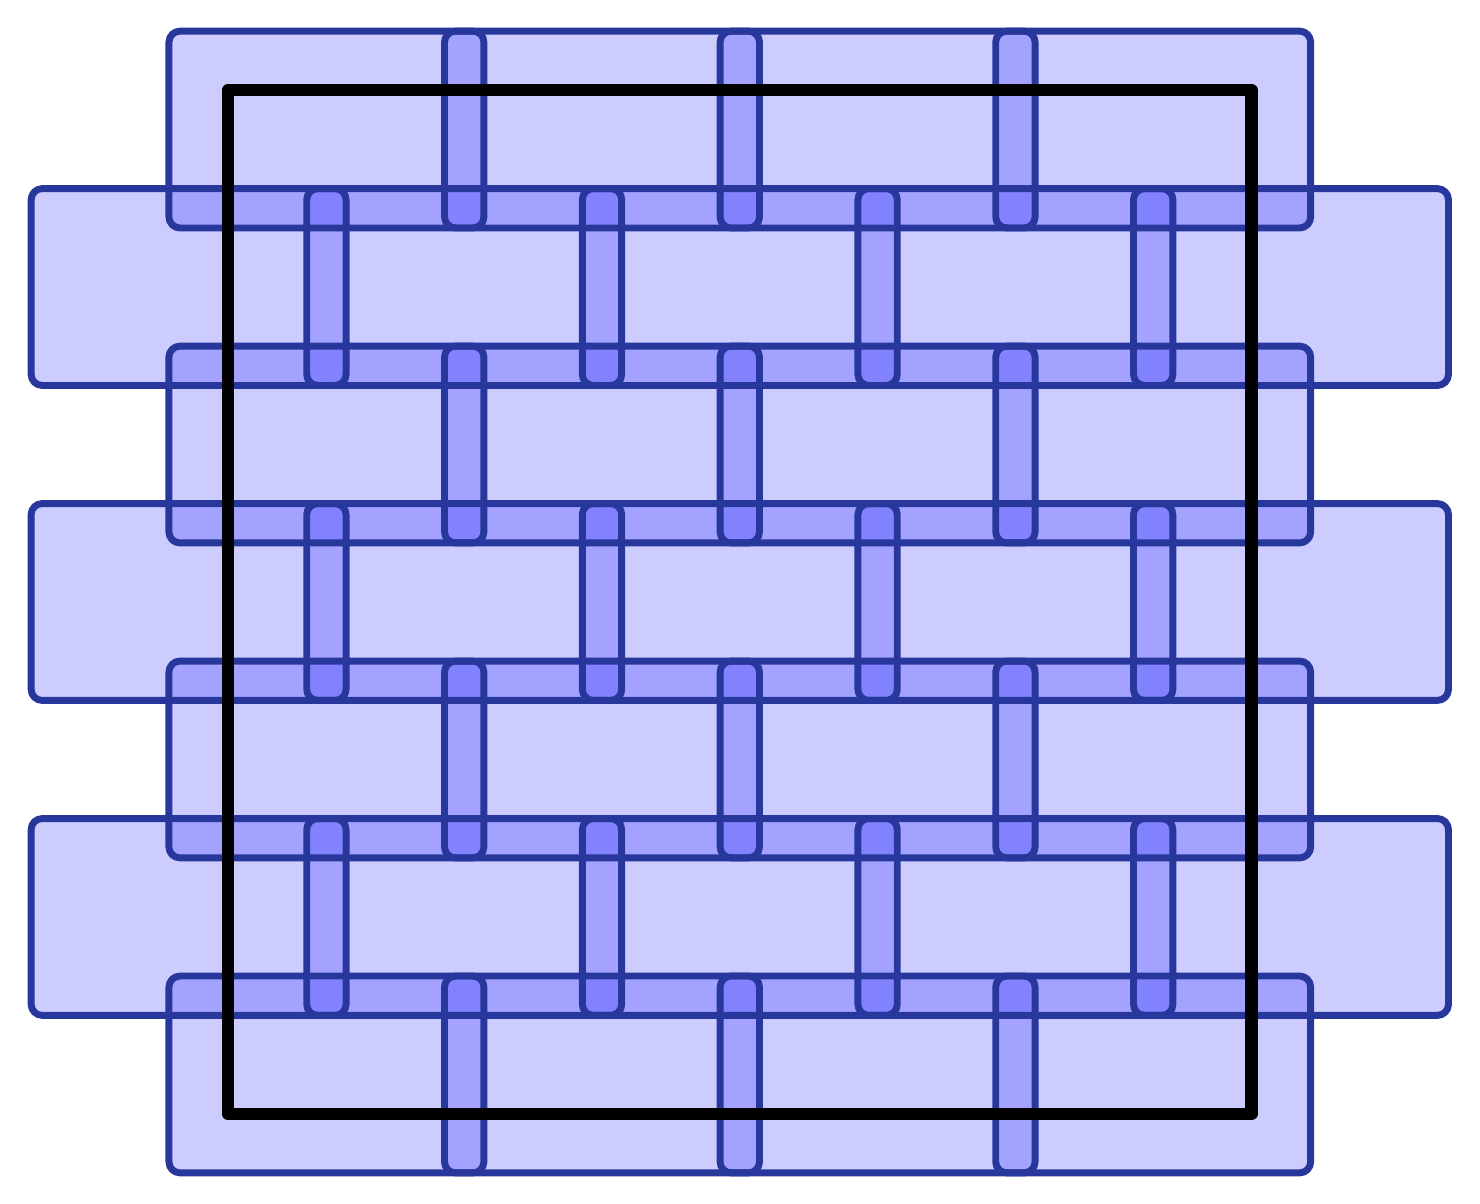
\begin{tikzpicture}[
    line width=2.5pt,
    line join=round,
    line cap=round,
    lightblock/.style={
        fill=blue!100,
        opacity=0.2,
        rounded corners=4pt
    },
    drawblack/.style={
        draw=darkBlue,
        rounded corners=4pt
    }
]

    \coordinate (P1) at (0,0);
    \coordinate (P2) at (4, 2.5);
    \coordinate (V1) at (1.75, -2);
    \coordinate (V2) at (3.5,0);
    \coordinate (V3) at (0,-4);
    % Define shapes / layers
    % Light cyan rectangles
    % Top wide rectangle

    % \foreach \i in {1,...,14} \node[colGreen, above left=2pt] at (R\i) {\Large $R_{\i}$};

    % \foreach \i in {1,...,14} {
    %     \foreach \j in {1,...,3} {
    %         \node[colGreen, above left=2pt] at (R\i\j) {\Large $R_{\i,\j}$};
    %     }
    % }

    \foreach \i in {1,...,4} {
        \foreach \j in {0,...,3} {
            \path[lightblock] 
            ($ (P1) + \i*(V2) + \j*(V3) $)
            rectangle
            ($ (P2) + \i*(V2) + \j*(V3) $);
        }
    }

    \foreach \i in {0,...,4} {
        \foreach \j in {0,...,2} {
            \path[lightblock] 
            ($ (P1) + (V1) + \i*(V2) + \j*(V3) $)
            rectangle
            ($ (P2) + (V1) + \i*(V2) + \j*(V3) $);
        }
    }

    \foreach \i in {1,...,4} {
        \foreach \j in {0,...,3} {
            \path[drawblack] 
            ($ (P1) + \i*(V2) + \j*(V3) $)
            rectangle
            ($ (P2) + \i*(V2) + \j*(V3) $);
        }
    }

    \foreach \i in {0,...,4} {
        \foreach \j in {0,...,2} {
            \path[drawblack] 
            ($ (P1) + (V1) + \i*(V2) + \j*(V3) $)
            rectangle
            ($ (P2) + (V1) + \i*(V2) + \j*(V3) $);
        }
    }

    \draw[black, line width=4.5pt] (4.25,-11.25) rectangle (17.25,1.75);
    % \path[drawblack] (P1) rectangle (P2);
    % \path[lightblock] ($(P1) - (V1)$) rectangle ($(P2) - (V1)$);
    % \path[lightblock] ($(P1) - (V2)$) rectangle ($(P2) - (V2)$);
    % \path[lightblock] ($(P1) - (V3)$) rectangle ($(P2) - (V3)$);
    
\end{tikzpicture}
}